
\documentclass[12pt]{article}

\usepackage{amsmath}
\usepackage[margin=0.75in]{geometry}
\usepackage{graphicx}
\usepackage[colorlinks]{hyperref}
\allowdisplaybreaks

\begin{document}

\section*{Problema 1.1}

Para $P(B|A)$, la Figura~\ref{fig:1a} grafica las estimaciones numéricas 
usando distintos números de repeticiones (puntos azules), intervalos de
confianza del 99\% (barras de error) y el valor
analitico de esta probabilidad (linear horizontal punteada).
El script para generar esta figura esta
\href{https://github.com/joacorapela/delfiProbability2026/blob/master/code/scripts/doICD1a.R}{aca}.

Vemos que los intervalos de confianza cubren el valor analítico de $P(B|A)$
para todos los números de repeticiones y que a medida que el número de
repeticiones aumenta el largo de estos intervalos disminuye, indicando que la
variabilidad de las estimaciones disminuye.

\begin{figure}
    \centering
    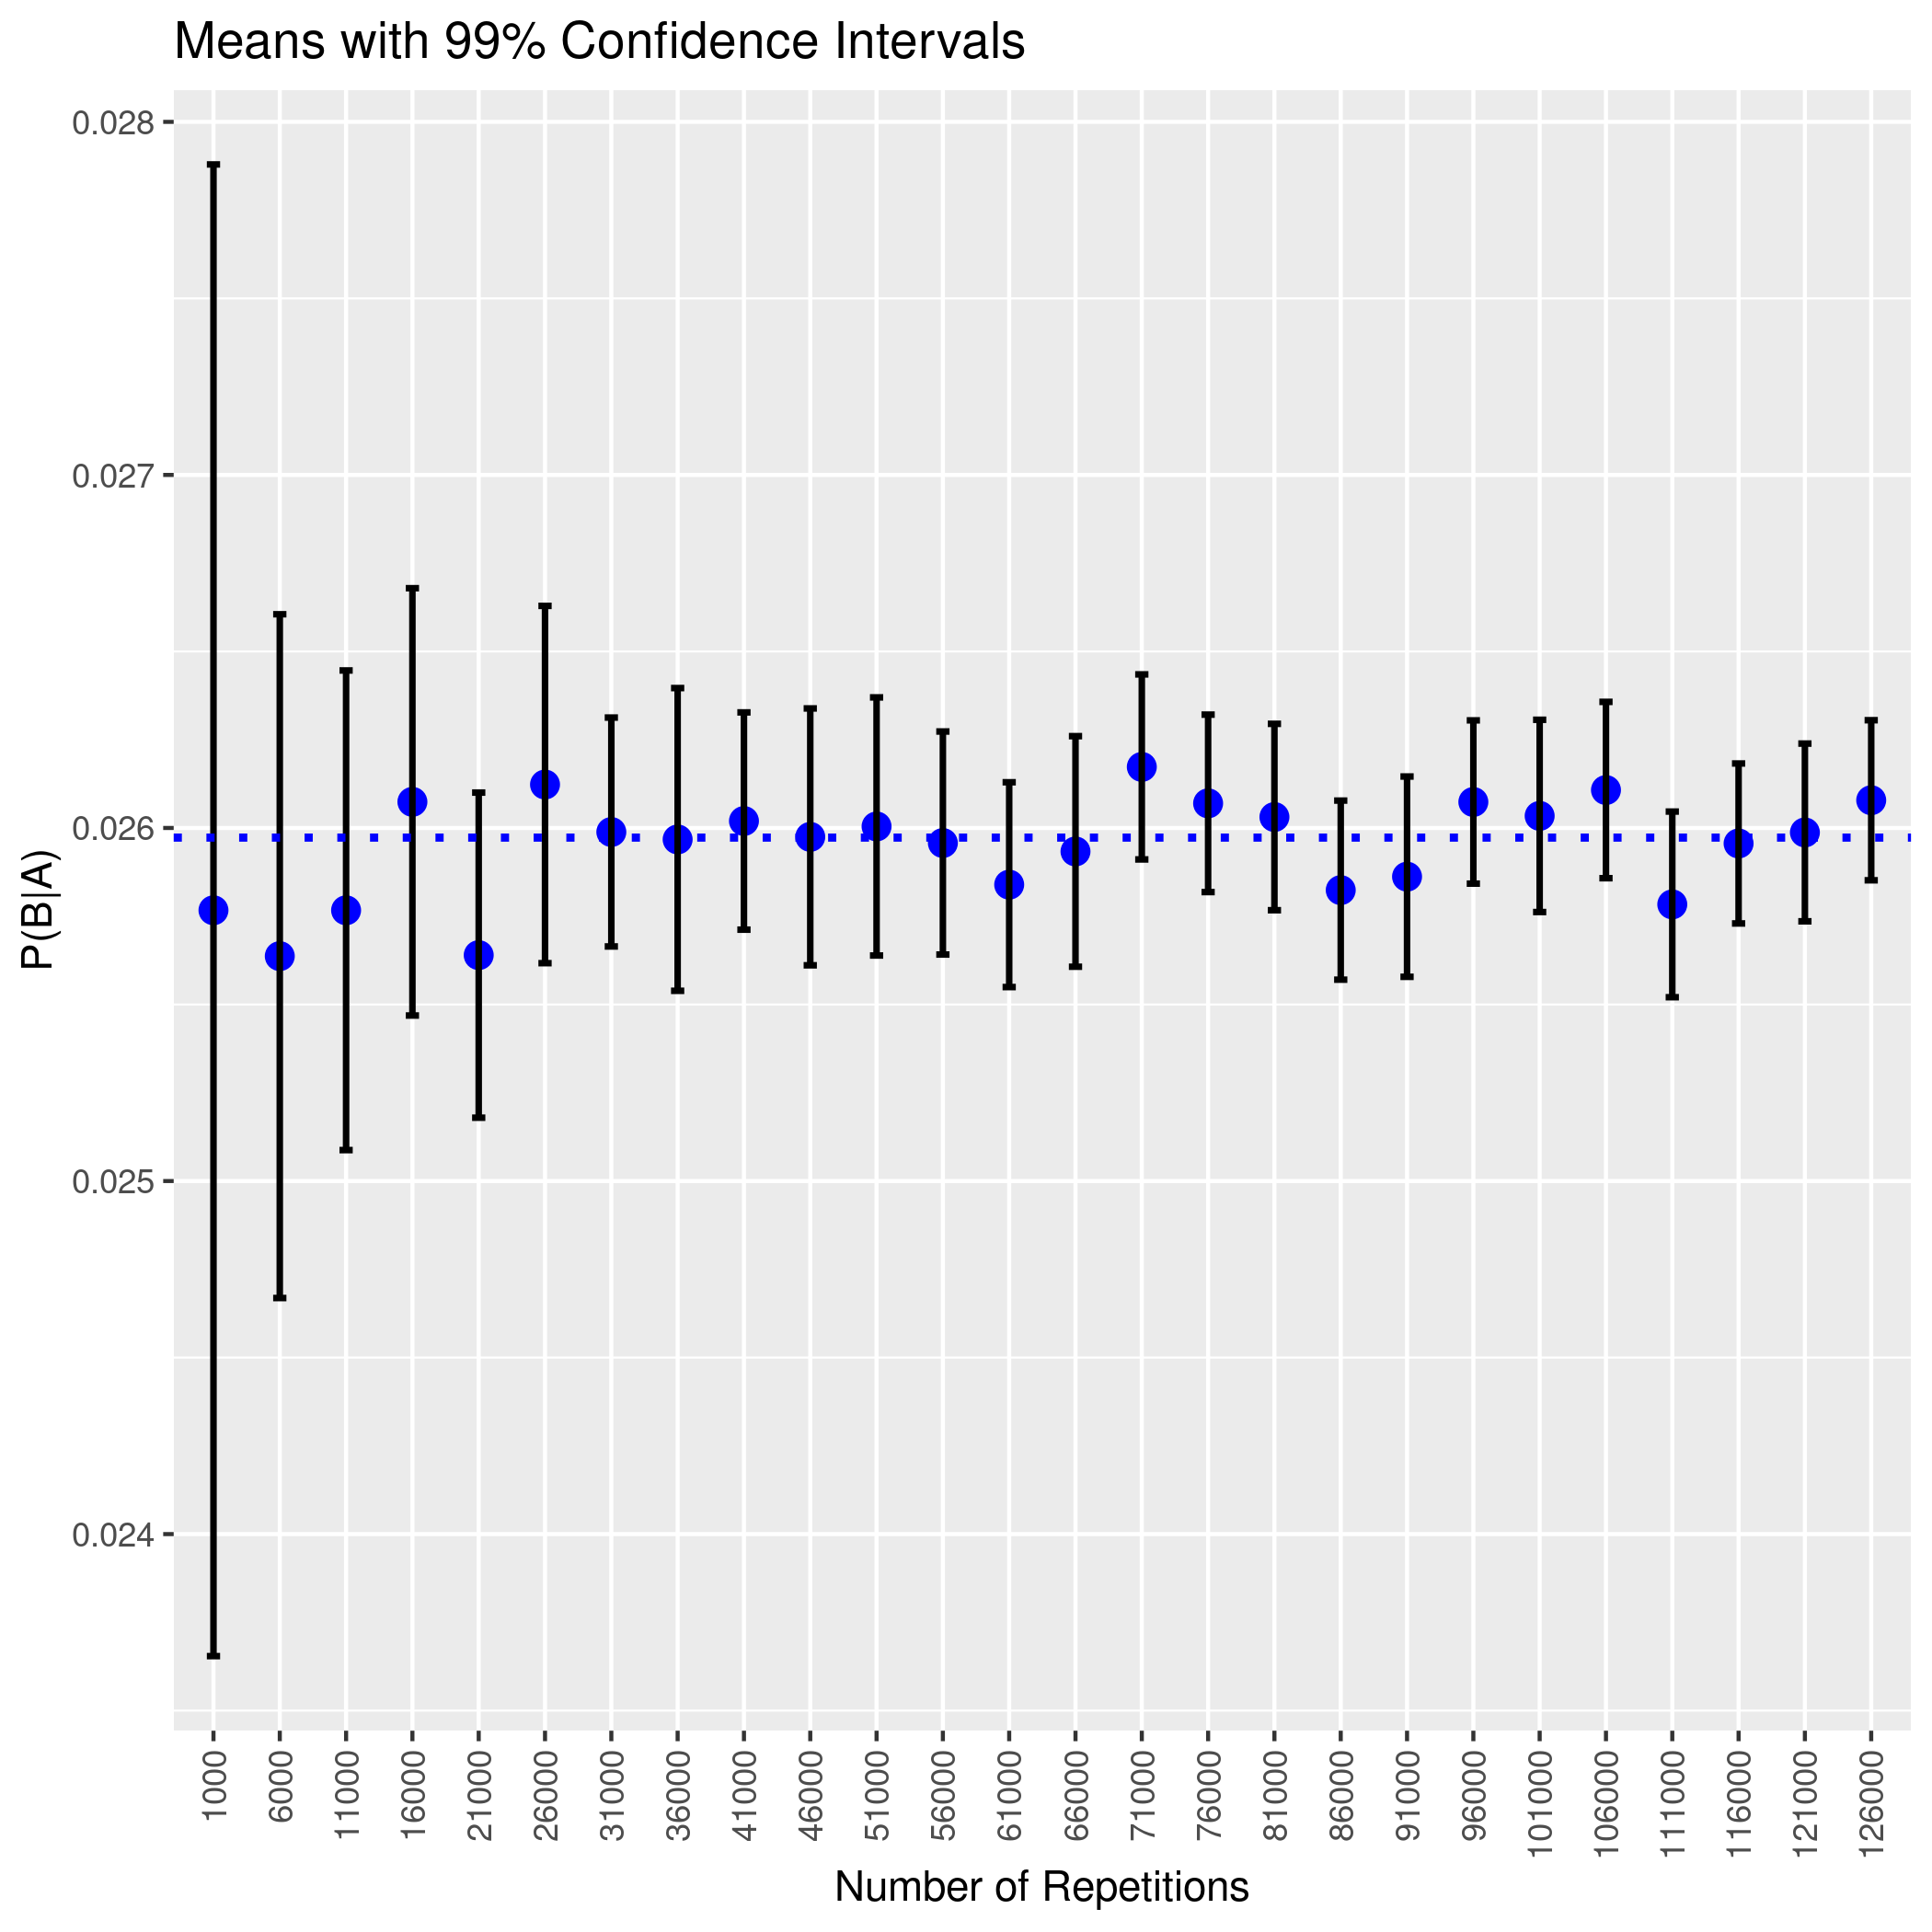
\includegraphics[width=6in]{../../figures/ICD1a.png}
    \caption{Estimación puntual de la probabilidad del evento B condicionado en el
    evento A, $P(B|A)$, e intervalo de confianza al 99\%.}
    \label{fig:1a}
\end{figure}

\subsection*{Derivación analítica de $P(B|A)$}

\begin{align*}
    P(B|A)&=\frac{P(A,B)}{P(A)}\\
    P(A,B)&=P(\text{``más atajadas que penales''}\cap\text{``ningún gol fuera del area''})\\
          &=P(\text{``5 atajadas''})+P(\text{``4 atajadas y 1 penal''})+P(\text{``3 atajadas y 2 penales''})\\
    P(\text{``5 atajadas''})&=P([A,A,A,A,A])\\
    P(\text{``4 atajadas y 1 penal''})&=P([A,A,A,A,P])\frac{5!}{4!}\\
    P(\text{``3 atajadas y 2 penales''})&=P([A,A,A,P,P])\frac{3!}{2!}\\
    P(A)&=P(A\cap(\text{``0 goles''}\cup\text{``1 gol''}\\
        &\cup\text{``2 goles''}\cup\text{``3 goles''}\\
        &\cup\text{``4 goles''}))\\
        &=P((A\cap\text{``0 goles''})\cup(A\cap\text{``1 gol''})\\
        &\cup(A\cap\text{``2 goles''})\cup(A\cap\text{``3 goles''})\\
        &\cup(A\cap\text{``4 goles''})))\\
        &=P(A\cap\text{``0 goles''})+P(A\cap\text{``1 gol''})\\
        &+P(A\cap\text{``2 goles''})+P(A\cap\text{``3 goles''})\\
        &+P(A\cap\text{``4 goles''})\\
    P(A\cap\text{``0 goles''})&=P(A,B)\\
    P([A,A,A,A,A])&=\frac{20}{64}\frac{19}{63}\frac{18}{62}\frac{17}{61}\frac{16}{60}\\
    P([A,A,A,A,P])&=\frac{20}{64}\frac{19}{63}\frac{18}{62}\frac{17}{61}\frac{10}{60}\\
    P([A,A,A,P,P])&=\frac{20}{64}\frac{19}{63}\frac{18}{62}\frac{10}{61}\frac{9}{60}\\
    P(A\cap\text{``1 gol''})&=P(\text{``mas atajadas que penales y 1 gol''})\\
                              &=P([A,A,A,A,G])\frac{5!}{4!}+P([A,A,A,P,G])\frac{5!}{3!}\\
    P([A,A,A,A,G])&=\frac{20}{64}\frac{19}{63}\frac{18}{62}\frac{17}{61}\frac{34}{60}\\
    P([A,A,A,P,G])&=\frac{20}{64}\frac{19}{63}\frac{18}{62}\frac{10}{61}\frac{34}{60}\\
    P(A\cap\text{``2 goles''})&=P(\text{``mas atajadas que penales y 2 goles''})\\
                              &=P([A,A,A,G,G])\frac{5!}{3!2!}+P([A,A,P,G,G])\frac{5!}{2!2!}\\
    P([A,A,A,G,G])&=\frac{20}{64}\frac{19}{63}\frac{18}{62}\frac{34}{61}\frac{33}{60}\\
    P([A,A,P,G,G])&=\frac{20}{64}\frac{19}{63}\frac{10}{62}\frac{34}{61}\frac{33}{60}\\
    P(A\cap\text{``3 goles''})&=P(\text{``mas atajadas que penales y 3 goles''})\\
                              &=P([A,A,G,G,G])\frac{5!}{3!2!}\\
    P([A,A,G,G,G])&=\frac{20}{64}\frac{19}{63}\frac{34}{62}\frac{33}{61}\frac{32}{60}\\
    P(A\cap\text{``4 goles''})&=P(\text{``mas atajadas que penales y 4 goles''})\\
                              &=P([A,G,G,G,G])\frac{5!}{4!}\\
    P([A,G,G,G,G])&=\frac{20}{64}\frac{34}{63}\frac{33}{62}\frac{32}{61}\frac{31}{60}
\end{align*}

\section*{Problema 1.2}

La Figura~\ref{fig:1b} grafica las estimaciones de la probabilidad del evento B
usando distintos números de repeticiones. También muestra para cada número de
repeticiones el intervalo de muestreo del 99\% de confianza. Cuando estimaciones de la probabilidad
del evento B se generan con datos sampleados bajo la hipótesis nula, estas
estimaciones caerán en el intervalo de muestreo del 99\% de confianza con una probabilidad del 99\%.
El script para generar esta figura esta
\href{https://github.com/joacorapela/delfiProbability2026/blob/master/code/scripts/doICD1b.R}{aca}.

\begin{figure}
    \centering
    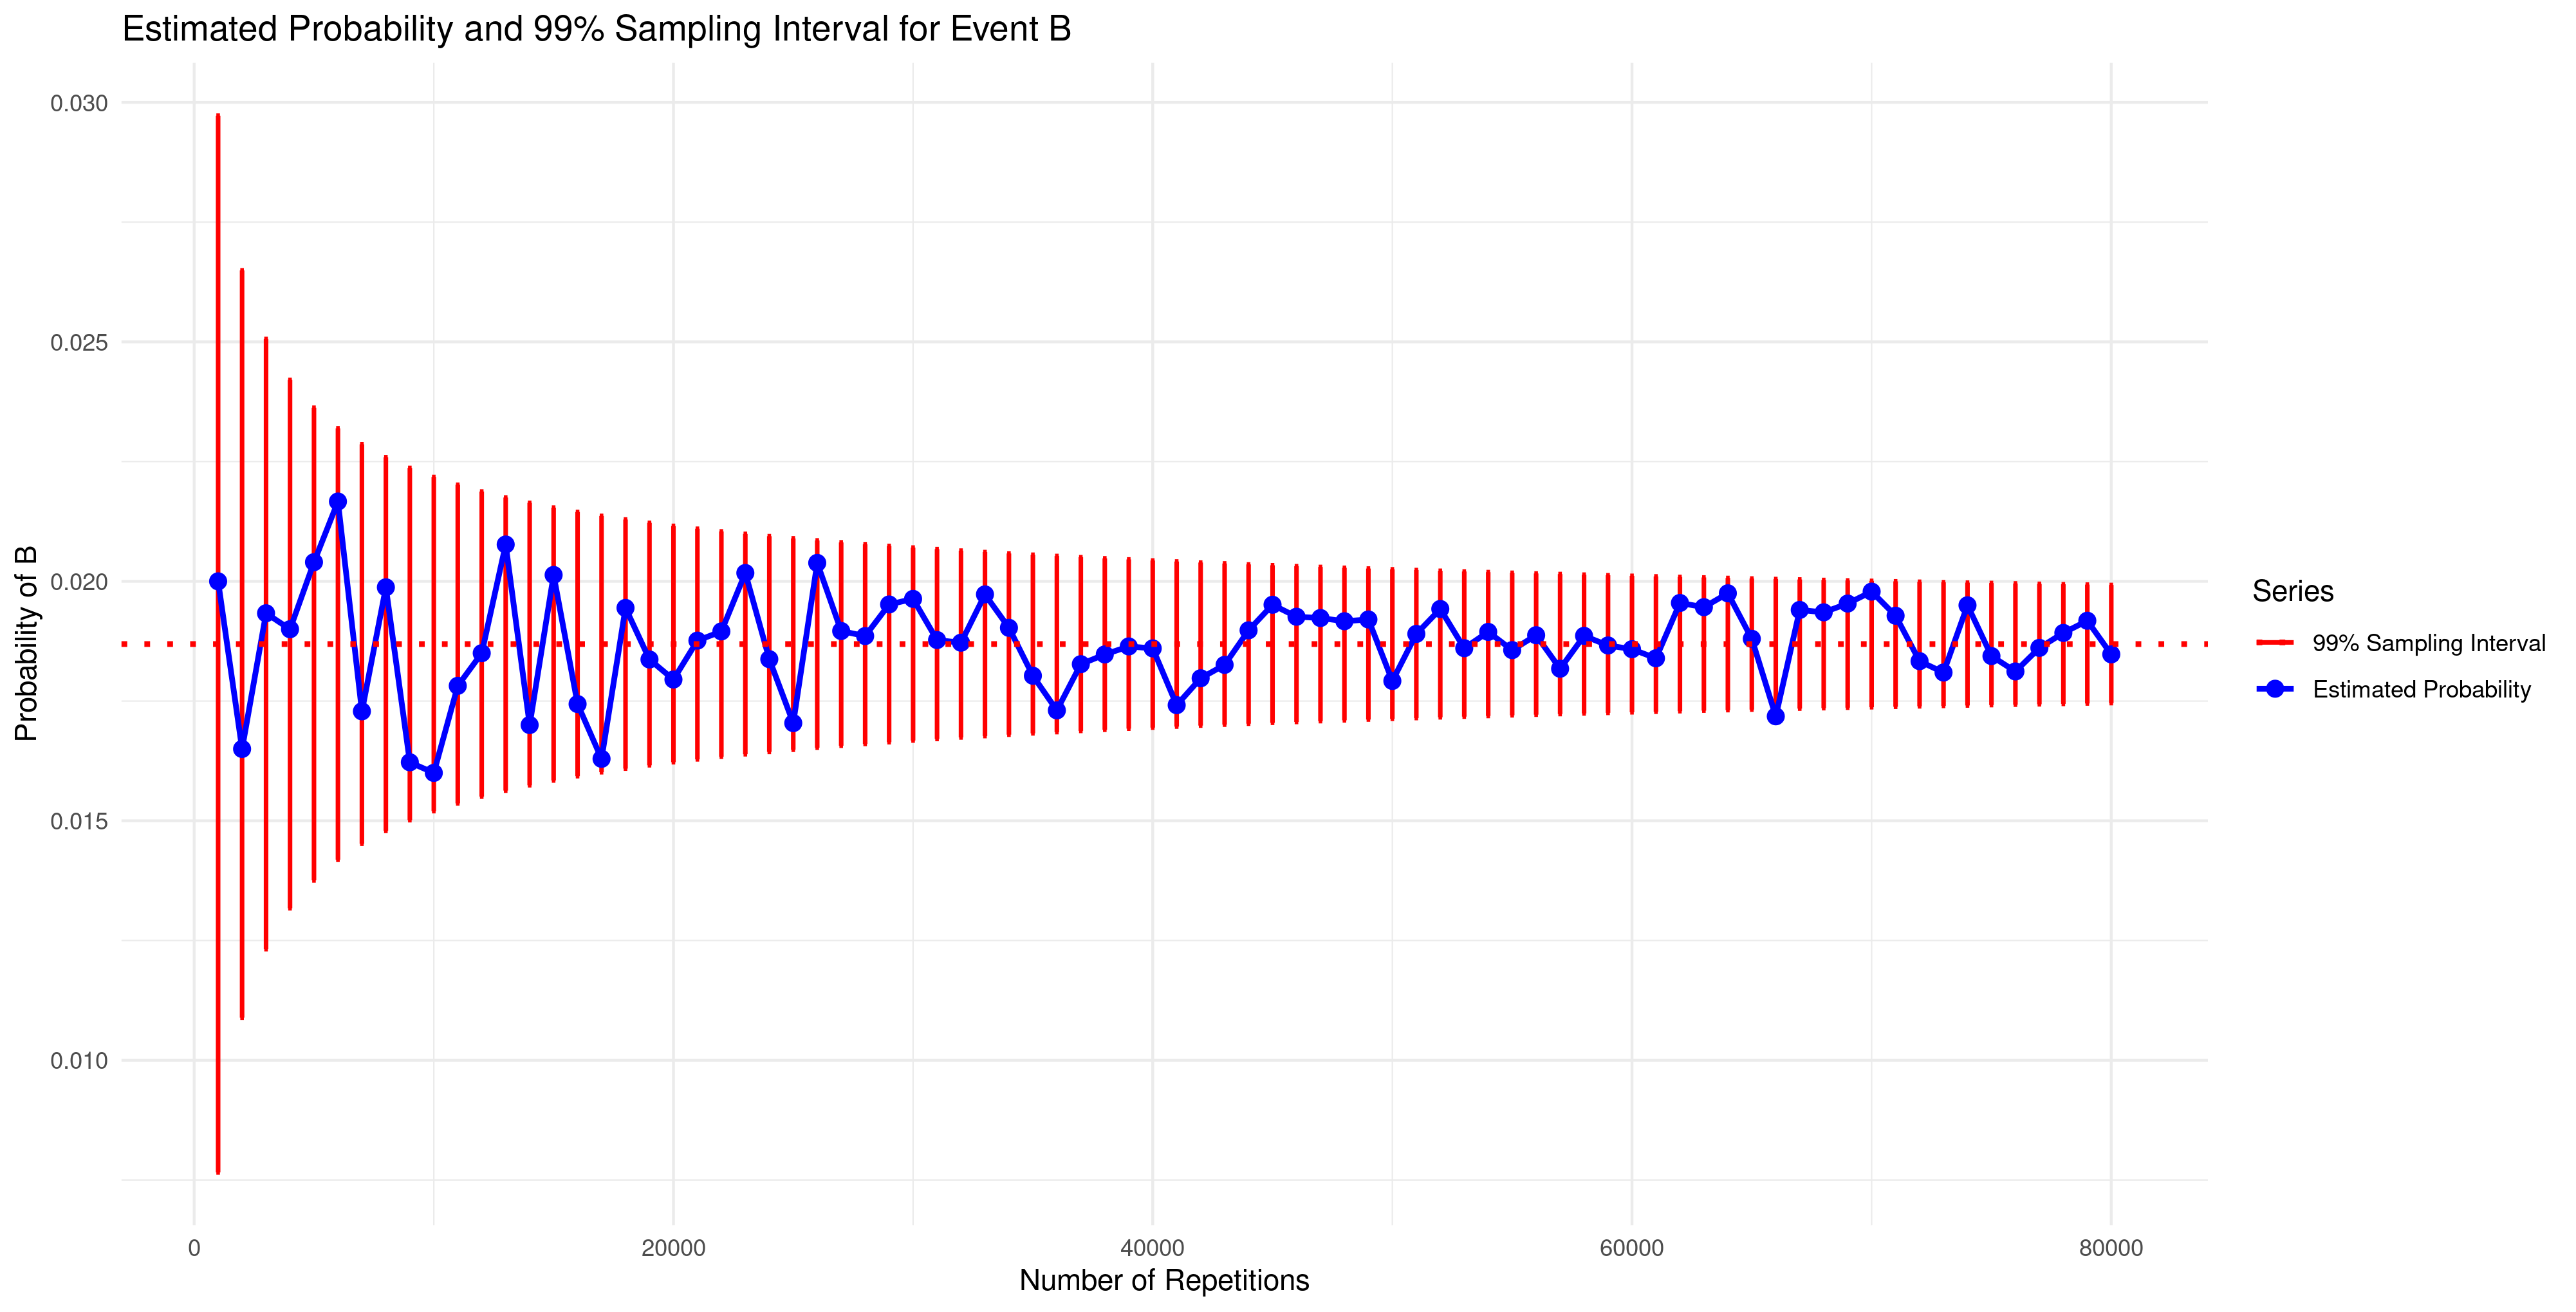
\includegraphics[width=6in]{../..//figures/ICD1b.png}
    \caption{Estimación de la probabilidad del evento B e intervalo de muestreo
    del 99\%.}
    \label{fig:1b}
\end{figure}

Para derivar la expresión del intervalo de muestreo, primero derivamos la
distribución del estimador de la probabilidad, $p$, del evento B. Con los datos
del problema:

\begin{align*}
    p=\frac{30\times 29\times 28\times 27\times 26}{64\times 63\times 62\times 61\times 60}
\end{align*}

Llamamos al estimator de $p$ con $N$ muestras como $\hat{p}_N$:

\begin{align*}
    \hat{p}_N=\frac{1}{N}\sum_{i=1}^NX_i
\end{align*}

\noindent donde las variables $\{X_i\}$ son variables independientes e
identicamente distribuidas con distribución Bernoulli con media $p$. La
variable $X_i$ tomará el valor 1 si en el muestreo $i$ el evento B ocurrió, y
el valor 0 en caso contrario. Es decir,

\begin{align*}
    X_i\sim Bernoulli(p)
\end{align*}

Sabemos que $E\{X_i\}=p$ y $Var\{X_i\}=p(1-p)$. Entonces

\begin{align*}
    E\left\{\hat{p}_N\right\}&=\frac{1}{N}\sum_{i=1}^NE\{X_i\}=\frac{1}{N}\sum_{i=1}^Np=p\\
    \text{Var}\left\{\hat{p}_N\right\}&=\frac{1}{N^2}\sum_{i=1}^N\text{Var}\{X_i\}=\frac{1}{N^2}Np(1-p)=\frac{p(1-p)}{N}
\end{align*}

Ahora, por el Teorema Central del Límite, para N suficientemente grande, se
cumple que

\begin{align}
    \hat{p}_N\sim\mathcal{N}\left(\mu=p,\sigma^2=\frac{p(1-p)}{N}\right)\label{eq:estimator}
\end{align}

Entonces

\begin{align*}
    Z=\frac{\hat{p}_N-\mu}{\sigma}\sim\mathcal{N}(0, 1)
\end{align*}

Por lo cual

\begin{align*}
    P(-z_{\alpha/2}\le Z<z_{\alpha/2})&=1-\alpha\\
    P(-z_{\alpha/2}\le\frac{\hat{p}_N-\mu}{\sigma}<z_{\alpha/2})&=1-\alpha\\
    P(\mu-\sigma z_{\alpha/2}\le\hat{p}_N<\mu+\sigma z_{\alpha/2})&=1-\alpha
\end{align*}

La última ecuación nos dice que, para $N$ suficientemente grande, con una
probabilidad de $1-\alpha$ nuestro estimador de la probabilidad del evento B
estará en el intervalo de muestreo $[\mu-\sigma z_{\alpha/2},\mu+\sigma
z_{\alpha/2}]$, donde $\mu$ y $\sigma$ están dadas en Eq.\ref{eq:estimator}.

\end{document}
